\section{序論}
\label{ch:introduction}

現代において、ニュースといった情報の入手と拡散が簡単にできるソーシャルメディアは生活の重要な一部となった。
その中には信憑性に乏しい情報が含まれており、特に悪意によって読者を騙して誤った風説を作るために作られた情報であるフェイクニュースがある。

フェイクニュースの実例として、特に今年は新型コロナウイルス感染症(COVID-19)にまつわる誤った風説がソーシャルメディア上で広く流布された。
WHO局長はこの問題を``インフォデミック''と呼び、フェイクニュースはウイルスそのものよりも早く簡単に拡散されると警戒を呼びかけている。\cite{ZAROCOSTAS2020676}
また、フェイクニュースによってオンライン上で誤った風説が広がった結果、オフライン上へ大きな影響を与えたこともある。
ワシントンDCで発生したピザ屋で銃乱射事件が発生した際、被疑者はインターネット上でのフェイクニュースに端を発する児童ポルノ疑惑が犯行の動機であることが報道されている\cite{agencies_2016}。
以上より、フェイクニュースの拡散によって読者が事実に基づく正しいニュースへのアクセスが難しくなるため、民主主義の根幹を揺るがしてしまう。
現在、フェイクニュース検出に向けて有識者が事実関係を確認して結果を公表するファクトチェックが行われている。

\begin{figure}[t]
    \centering
    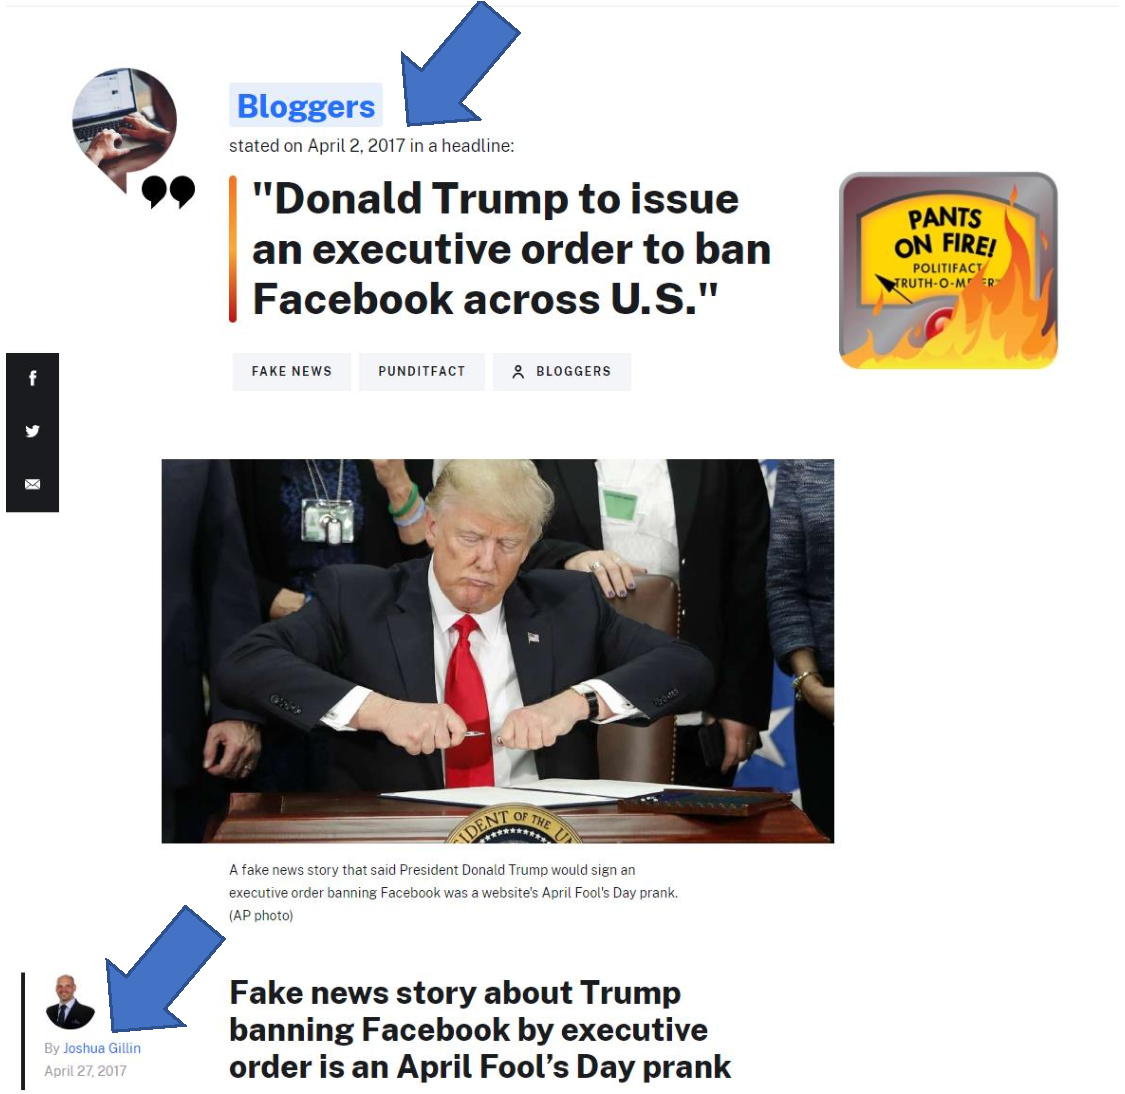
\includegraphics[width=\linewidth]{images/fact-check.pdf}
    \caption{
        北米で行われたファクトチェックの一例。
        % この情報はエイプリルフールで投稿された虚偽情報としている。
        青矢印はフェイクニュース投稿日時とファクトチェック結果投稿日時を示し、両者には25日もの間が開いている。
        }
    \label{fig:example}
\end{figure}

図\ref{fig:example}はファクトチェックの一例である\cite{gillin_2017}。
この実例のように、ファクトチェックは属人的な作業であることに加えて結果公表まで時間がかかるため、
フェイクニュースそのものに比べて拡散されにくい。
このため、機械学習によってフェイクニュースを自動で検出する研究が行われている。

自動検出にあたって困難な点は、フェイクニュースは人々を騙すために巧妙なつくりをしていることが挙げられる。
このため、単純なルールベース手法による検出は難しい。
検出性能の向上において、記事そのものがもつ情報に加えてソーシャルメディア上での反響を示すソーシャルコンテキスト(リツイート・いいね・リプライなど)
を考慮することが有効であることが先行研究で示されている\cite{Guo:2018:RDH:3269206.3271709}。
しかしながら、ソーシャルコンテキストはユーザの拡散によって生まれるため、この場合も早期の検出には向かない。
これに対して、ニュースに対してソーシャルメディア上で寄せられるコメントで発生しやすい単語を、条件付き変分オートエンコーダ(CVAE)で生成する手法も提案されている\cite{ijcai2018-533}。
この手法は、記事から確率分布とラベルを元に隠し変数を介して生成を行っている。

本研究では、記事と実際に記事に寄せられたコメントから信憑性の学習を行い、記事と限られた数のコメントから別のコメントを予測させた上で真偽を判断するモデルを提案する。
このモデルは、フェイクニュースそのものを生成するモデル\cite{NIPS2019_9106}を拡張する形で実装することでコメントの生成を実現する。
学習では記事と実際に記事に寄せられたコメントを3件、更に真偽ラベルを入力するが、テスト時は記事に加えて実際に寄せられたコメントは2件に制限し、真偽ラベルは入力しない。

我々は提案モデルの検出性能を実際に投稿された情報をもつデータセットによって検証した。
